\section{Design \& Implementation}
Swink discussed different ways to modulate the player avatar movement in \textit{Response Metrics} \cite{swink}. Inspired by ADSR envelopes (Attack-Decay-Sustain-Release), which are often used in order make an electronic musical instrument mimic the sound of a mechanical instrument \cite{adsr}, he proposed the idea of using velocity modulation to change the game feel. By altering the attack and release phase (or, acceleration and deceleration), it is possible to create different game feel, as illustrated by Figures \ref{fig:adsr_stiff} and \ref{fig:adsr_loose}.


%, e.g., the sound of a pipe organ or a guitar string. This is achieved by modulating the amplitude over time.

%Inspired by Swink's discussion about \textit{Response Metrics} \cite{swink}, a 2D platforming game was developed. The game changes two types of parameters between each round: how fast the ball accelerates and how fast it decelerates when moving horizontally. Swink calls these the \textit{attack} and \textit{release} phases, or, the acceleration and deceleration of avatar movement. Hence, the velocity of the player's avatar is modulated over time, creating different types of game feel. Figures \ref{fig:adsr_stiff} and \ref{fig:adsr_loose} show two examples of the modulations proposed by Swink.


%According to Swink, when the acceleration or deceleration is very long (e.g., the avatar takes more than 100 milliseconds to be perceived to be moving), the impression of instantaneous response erodes. Even if there are small changes in the velocity, if these cannot be perceived by the player, the game might feel unresponsive \cite{swink}. This is illustrated by Figure \ref{fig:adsr}.

\begin{figure}[htbp]
\centering
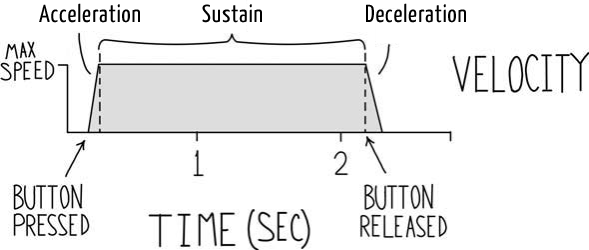
\includegraphics[width=0.40\textwidth]{Pics/adsr_stiff}
\caption{Short acceleration/deceleration gives a responsive, but stiff, feel. Figure inspired by Swink \cite{swink}.}
\label{fig:adsr_stiff}
\end{figure}

\begin{figure}[htbp]
\centering
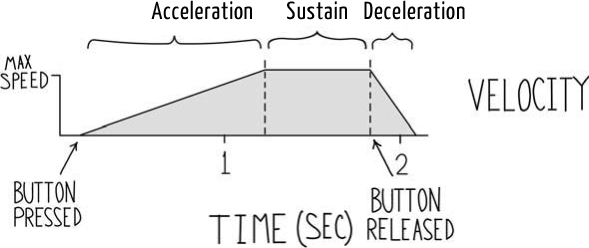
\includegraphics[width=0.40\textwidth]{Pics/adsr_loose}
\caption{Long acceleration gives a loose, but fluid, feel. Figure inspired by Swink \cite{swink}.}
\label{fig:adsr_loose}
\end{figure}

Taking inspiration from Swink, a game has been developed with this concept in mind. The game changes two types of parameters between each round: how fast the ball accelerates and how fast it decelerates (when moving horizontally). Hence, the velocity of the player's avatar is modulated over time. This means that when the player presses the movement button, the ball will take a certain amount of time before it reaches its maximum velocity. The same is applied when the player releases the button: the ball will gradually slow down, until it stops.


\begin{figure}[htbp]
\centering
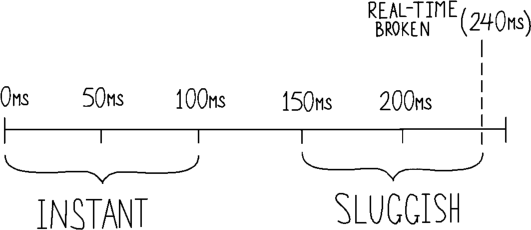
\includegraphics[width=0.40\textwidth]{Pics/response}
\caption{Model of response time and player perception. Depending on how big a delay there is from the player triggering an event to getting feedback, the game will gradually feel less responsive. Figure inspired by Swink \cite{swink}.}
\label{fig:response}
\end{figure}

%%% This is how to insert a table %%%
\begin{table}[htbp]
\centering
\begin{tabular}{|c|c|}
\hline \textbf{Fast}
& \textbf{Slow}\\\hline
[1 ms - 240 ms]
& [241 ms - 1500 ms]
\\\hline
\end{tabular}
\caption{Time intervals for the acceleration/deceleration.}
\label{tab:time}
\end{table}

Two intervals were chosen, inspired by Swink's model of player perception and feedback (see Figure \ref{fig:response}). The first interval, \textit{fast}, is between 1 millisecond and 240 milliseconds (staying within the limits of real-time perception). The second interval, \textit{slow}, is from 241 milliseconds to 1500 milliseconds (see Table \ref{tab:time}). For each round in the game, the player is assigned randomly-chosen time values within the two intervals. The reason for choosing random values instead oft fixed values is that it isn't perfectly clear at what exact point a game goes from feeling responsive to unresponsive (it's a gradual scale, as shown in Figure \ref{fig:response}). Additionally, the model in Figure \ref{fig:response} depicts the perception of getting discrete feedback, e.g., clicking on a button turns on a light bulb after 50 milliseconds. In the case of avatar movement, there is continuous stream feedback while the player is holding the movement button, since the avatar is gradually moving forward. However, if the acceleration/deceleration time is very big, the avatar will take some time before it gathers a velocity that can be perceived by the player. In other words, the time values change the total amount of time it takes from when a player presses a button to when the avatar reaches its maximum velocity (or, when releasing the button, reaches a velocity of zero). The acceleration/deceleration is thus scaled depending on the time values, using Equation \ref{eq:erl}.

% source: http://www.calculatorsoup.com/calculators/physics/velocity_a_t.php
\begin{equation} \label{eq:erl}
a = (v - v_0)/t
\end{equation} 
where $v_0$ is the initial velocity, $v$ is final (maximum) velocity, $a$ is the acceleration/deceleration and $t$ is the time.

Since there are two parameters, the acceleration and deceleration, there are four possible combinations, as shown in Table \ref{tab:combinations}. Additionally, there are 16 different order combinations (4x3x2x1)

%%% This is how to insert a table %%%
\begin{table}[htbp]
\centering
\begin{tabular}{|c|c|}
\hline \textbf{Acceleration}
& \textbf{Deceleration}\\\hline
Fast
& Fast
\\\hline
Slow
& Slow
\\\hline
Fast
& Slow
\\\hline
Slow
& Fast
\\\hline
\end{tabular}
\caption{Four different combinations.}
\label{tab:combinations}
\end{table}

%only sporadic work has been conducted in order to measure game feel \cite{feelBetter}.